
\chapter{Introduction} \label{sec:introduction}

In 2010 Gartner estimated the global accumulated Technical Debt (TD) to be US\$ 500 billion \cite{costOfTechnicalDebt} and that it has the potential to double by the end of 2015. These numbers give an insight of the relevance of this subject that lately, as shown in Figure \ref{fig:technical_debt_trend}, started to gain Practitioners' attention.

Technical Debt is a metaphor borrowed from the financial world used to described short time expedients and the adoption of sub-optimal decisions which inflate software cost over time \cite{first_mention_of_TD}. As in financial debt, Technical Debt is tied with the concept of Interest (also called Principal). It represents the difference in cost needed to successfully maintain the current solution and an optimal one \cite{technicalDebtInterest}. Moreover, Technical Debt has a third component that represents the probability of the debt to incur.

As described in \cite{mapping_study_td, exploration_of_td, exploration_of_td2}, Technical Debt accrues in every aspect of the Software's life-cycle and side effects of correlations between these different sub-dimension are often hard to identify and/or quantify. In addition, even within a specific dimension, TD tends to change based on the metric in use and these results might not be correlated \cite{4_methods_to_identify_td}.

Moreover, as highlighted in Chapter \ref{sec:related_work}, the available body of knowledge fails to identify similarities and differences between these dimensions. In particular, there are no prior studies about framing the problem of Test Code Quality within the available Technical Debt frameworks despite having other studies highlighting these kinds of problems \cite{gui_scripts_bad_smells,pitfalls_in_introducing_regression_testing}.

However, a simplistic map of the available knowledge about Source Code Technical Debt to Test Code don't consider Testware's specific aspects; i.e.\ in the Software Development pipeline testing activities come after developing ones and serve different purposes. Furthermore, Maintenance Activities on test code base are triggered by more factors. Namely: 1) Requirements, 2) Requirements that interest the Software Source Code, 3) Refactoring of Software Source Code, and 4) Refactoring of the available test-suite. In addition, Test Code is ubiquitous since it spans from function to system level and covers everything in-between. Additionally, the gaining traction of test automation require test suites to be more resilient towards Software Changes to not interrupt quality assurance processes. Consequently, the available knowledge on identifying and quantifying Technical Debt will result in underestimate assessment of both debt and repayment of the the Interest.

Therefore, considering that Testing uses between 40\% and 80\% of the available resources \cite{exploratorying_testing_td}, it is clear that providing a better understanding of technical debt accretion within testware is important. The findings of this study can act as stepping stone torwards quantitative models that can be integrated in broader frameworks for calculating and managing Technical Debt (e.g.\ SONAR \cite{sonar_evaluate_td}).

For these reasons and considering the knowledge gaps highlighted by several secondary studies, i.e.\ \cite{mapping_study_td, exploration_of_td, exploration_of_td2}, that are extensively analyzed in Section \ref{sec:related_work}, the following Research Questions were crafted in order to shed light on the mentioned problem:

\begin{itemize}
    \itemsep0em

    \item \textbf{RQ1:} To what extent the Source Code Technical Debt reported in \cite{mapping_study_td} is applicable to Testware?

    \item \textbf{RQ2:} What are the Testware Technical Debt items that are unique to Test Source Code?

    \item \textbf{RQ3:} For the elements identified in RQ1 and RQ2, what is the related Interest according to Studies analyzed in \cite{mapping_study_td}?

\end{itemize}

\begin{figure}[h]
\centering
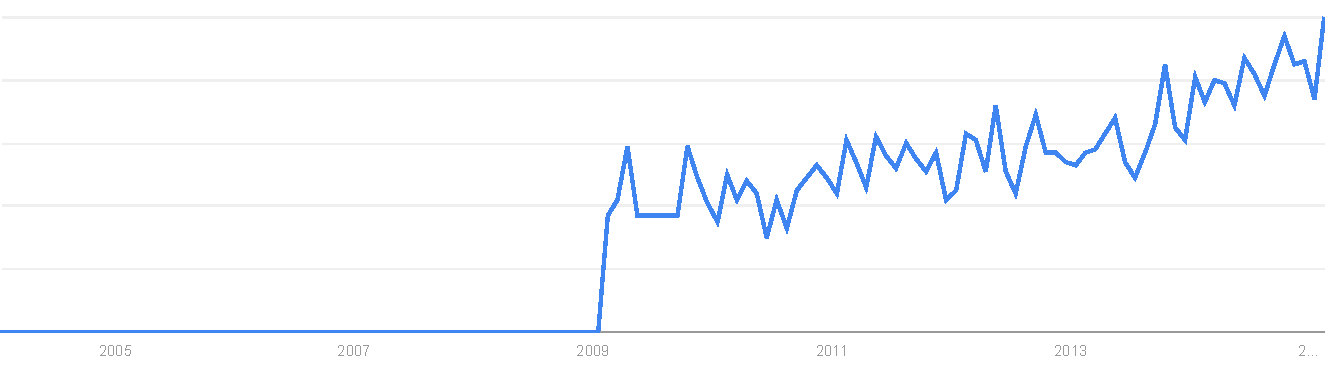
\includegraphics[width=\textwidth]{figure/technicalDebt.pdf}
\caption{Popularity of \textit{Technical Debt} in Google over time.}
\label{fig:technical_debt_trend}
\end{figure}



To answer these questions, an Exploratory Case Study was conducted in Industry settings. The company under study is a large multinational software-house operating in the Aeronautical market, providing solutions for managing crews, personnel and assets' maintenance to airline companies. A detailed analysis of the Company, its processes and the Case under analysis is provided in Section \ref{sec:case-description}.

The report is articulated as follows. Section \ref{sec:related_work} presents the relevant related work available to date on the topic. Section 3 contains an accurate description of the methods used withing this study. Section 4 illustrates the data that has been gathered which is subsequently analyzed and discussed in Section 5. Section 6 will discuss Threats to Validity and all the steps taken to lessen them. Finally, Section 7 contains the conclusion and list questions raised but not answered by this study.


